%This LaTex template file was provided my D. Kevin McGrath
%for use in CS 311 / CS 411

\documentclass[letterpaper,10pt,onecolumn,titlepage]{article}

\usepackage{graphicx}                                        
\usepackage{amssymb}                                         
\usepackage{amsmath}                                         
\usepackage{amsthm}
\usepackage{longtable}                                          

\usepackage{alltt}                                           
%\usepackage{float}
\usepackage{color}
\usepackage{url}

%\usepackage{balance}
%\usepackage[TABBOTCAP, tight]{subfigure}
%\usepackage{enumitem}
%\usepackage{pstricks, pst-node}


\usepackage{geometry}
\geometry{textheight=8.5in, textwidth=6in}

%random comment

\newcommand{\cred}[1]{{\color{red}#1}}
\newcommand{\cblue}[1]{{\color{blue}#1}}

\usepackage{hyperref}
\usepackage{geometry}
\usepackage[lofdepth,lotdepth]{subfig}

\def\name{Kyson Montague}

%% The following metadata will show up in the PDF properties
\hypersetup{
  colorlinks = true,
  urlcolor = black,
  pdfauthor = {\name},
  %Insert Keywords Here
  pdfkeywords = {ENGR 421, ``Applied Robotics''},
  pdftitle = {ENGR 421 Design Proposal},
  pdfsubject = {ENGR 421 Design Proposal},
  pdfpagemode = UseNone
}
\title{ENGR 421 Design Proposal}
\author{Kyson Montague}
%\institute{Oregon State University}
\begin{document}

\maketitle

\section{Introduction}
In order to successfully compete in a game of crossfire, a robot must be
able to track the target in real-time, find the optimal point on the target to
hit, and then aim and fire the projectile at the intended location on the
target.  There are several design considerations to keep in mind when
designing such a robot.  Since the game will be played in real-time against
an opposing robot, all components of the robot should be as fast as possible.
Additionally, various game-play strategies may result in differing outcomes (offensive vs defensive tendencies could change based on factors such as: remaining
ammunition, game time remaining, location of the puck(s), etc.).

The various attributes described above lead to a basic division of robot
functionality into three main blocks:
\begin{enumerate}
\item Targeting/Tracking Mechanism (Sense)
\item Game Decision Engine (Think)
\item Projectile Aim \& Fire Mechanism (Act)
\end{enumerate}

The Targeting/Tracking Mechanism is responsible for determining where the puck
is located at any given point in time.  As the puck moves, the tracking 
mechanism should adjust as quickly as possible.  The information from the
tracking mechanism will be fed into the game engine, which will be responsible
for determining the optimal target for the next BB.  The optimal location
may change through the duration of the game based on various factors such as
puck location, remaining ammunition, remaining time, etc. The game engine will
then feed the desired target vector information to the Aim and Fire mechanism,
which is responsible for translating the digital target information into the
physical action of firing the projectile.  

The interaction of each component is depicted graphically in Figure 
\ref{block_diag}, and is
discussed in more detail throughout the duration of this document.

\begin{figure}[h!]
  \centering
  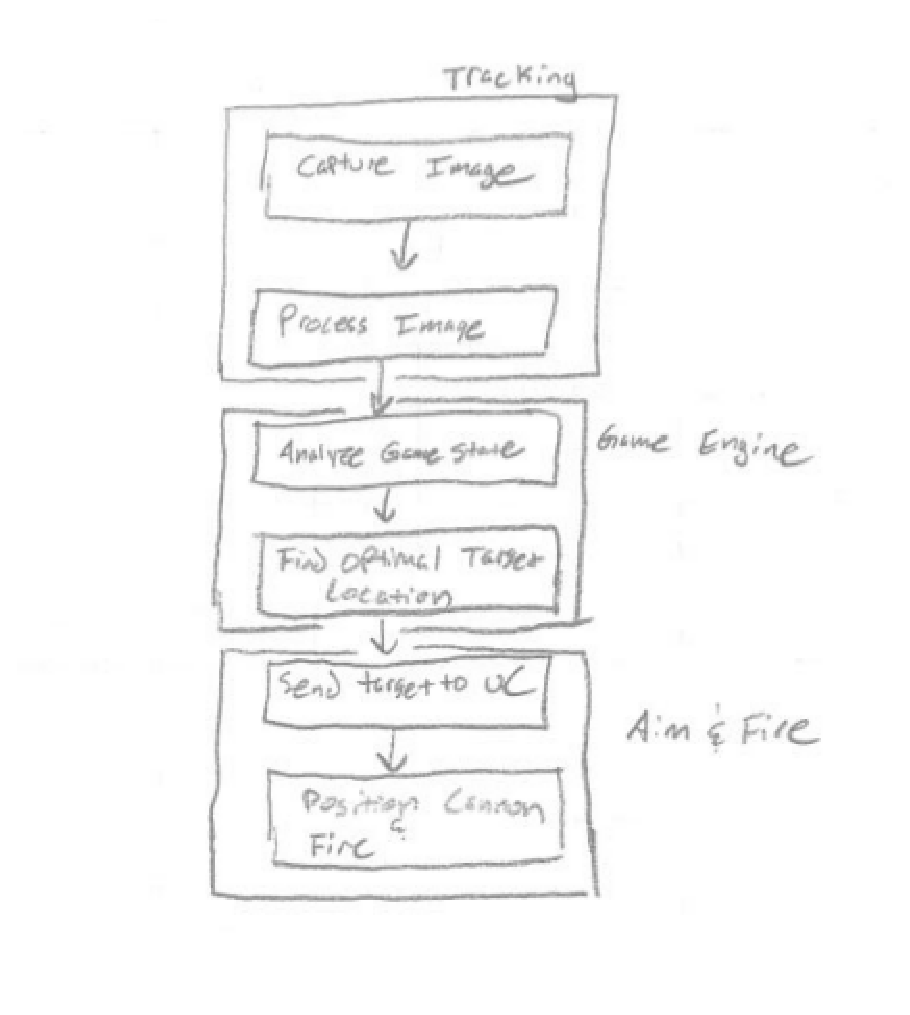
\includegraphics[width=0.5\textwidth]{./block_diag.eps}
  \caption{Simple block diagram showing component interactions.}
  \label{block_diag}
\end{figure}



\section{Design Details}
\subsection{Targeting/Tracking Mechanism}
The Targeting/Tracking mechanism is responsible for locating the puck within
the field of play at any given point in time.  There are several approaches
that can be taken to achieve this, each method having its own trade-offs.
Object tracking can be done using SONAR, LIDAR, or computer vision.  For the
scope of this project, computer vision will offer the most robust solution
because the puck will be resting close to the surface of the table, making it
difficult for LIDAR and SONAR sensors to differentiate the target from the
background.  Since the color, shape, and size of the puck will be known 
ahead of time, real-time computer vision tracking should be feasible.

The tracking mechanism consists of one (or possibly two) cameras placed
slightly above the field of play, and directly over the center of the robot,
as seen in Figure \ref{fig_sketch}.
From this location, the camera(s) will have a view of the entire playing field.
An image of the field can be captured, and then processed, resulting in the
location of the puck.  This location will then be passed to the game engine
for further processing.

\begin{figure}[h!]
  \centering
  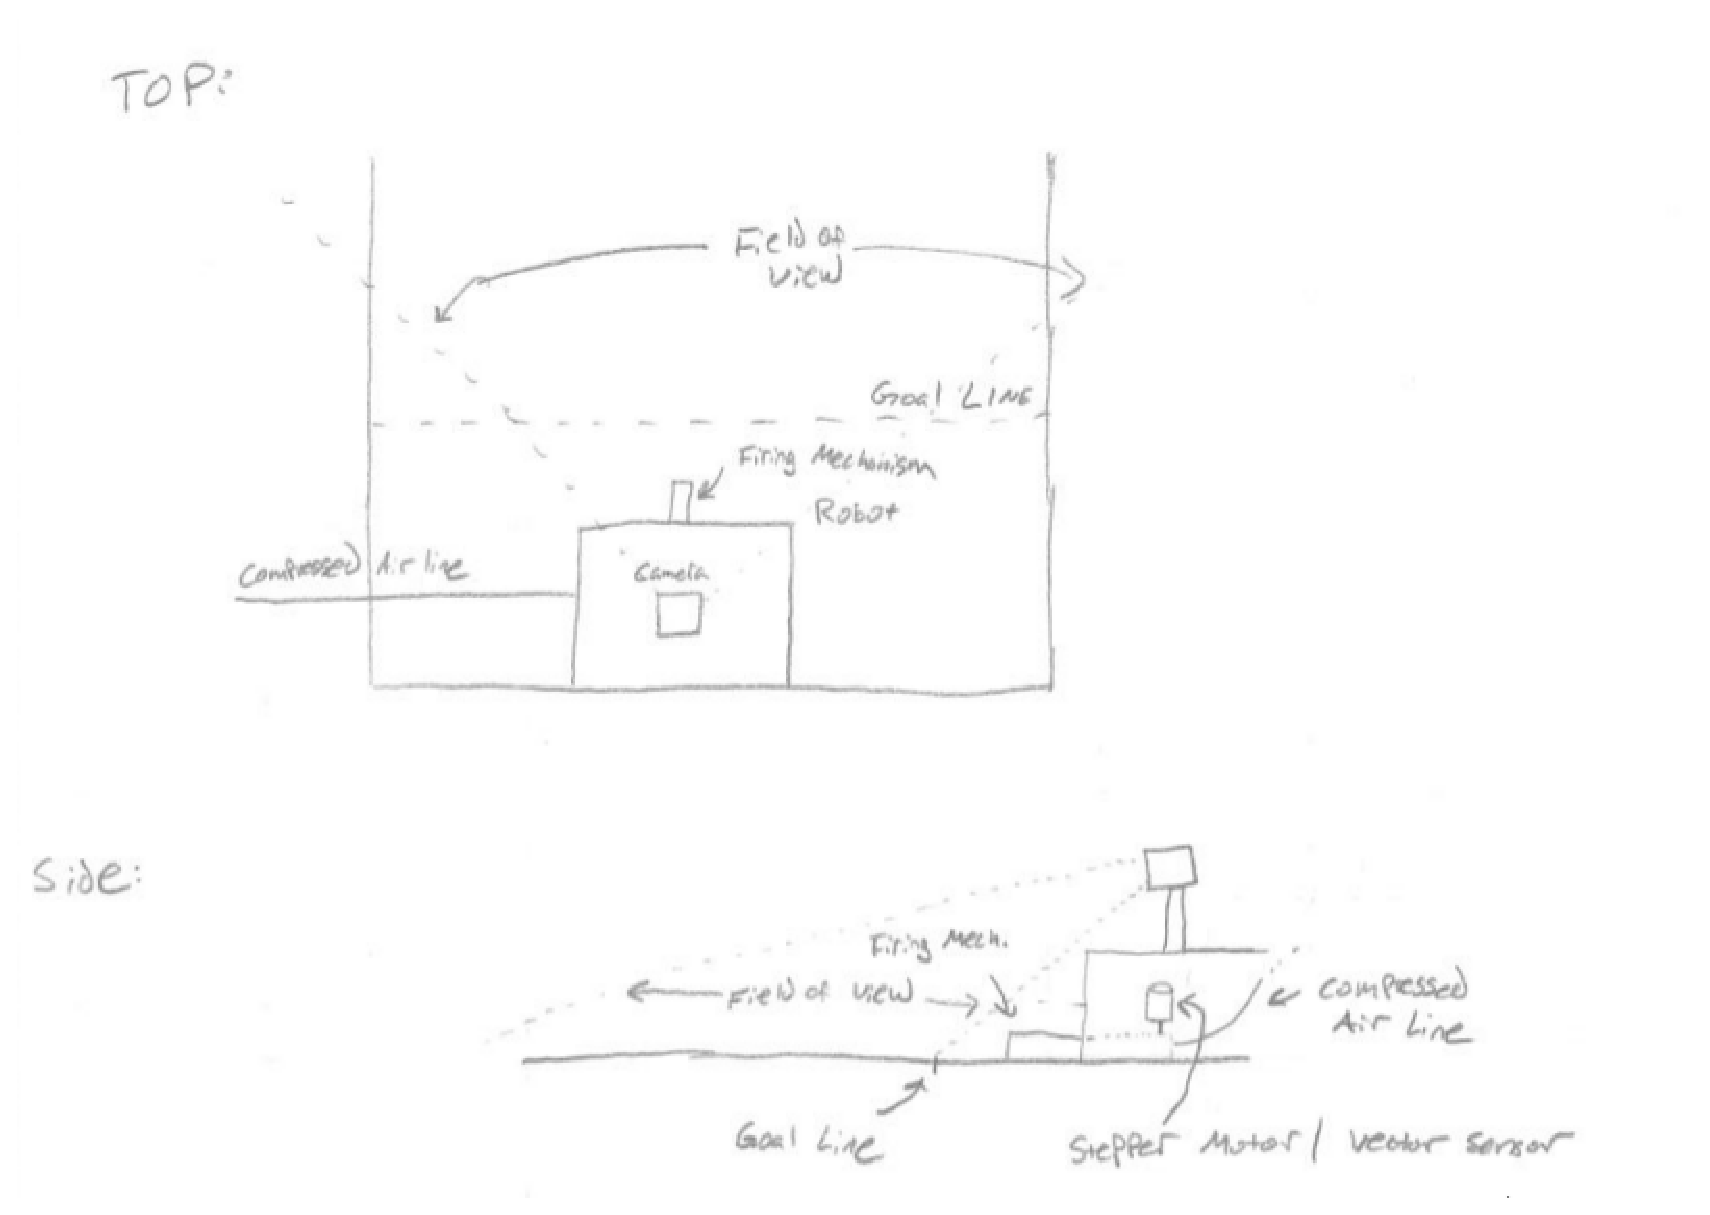
\includegraphics[width=0.8\textwidth]{./top_view.eps}
  \caption{Top and side view of robot mounted on playing field}
  \label{fig_sketch}
\end{figure}



\subsection{Game Decisions Engine}
The Game Decision Engine is responsible for taking the current location of the
puck, and computing the optimal target for the next BB.  Various factors
will affect the location of the next shot.  Under normal circumstances, the
optimal target will be the center of the puck.  However, as the puck moves
around the playing field and resources (ammo, time) begin to dwindle the
optimal target will change.  Many of these tweaks will come from actual testing
after the robot has been built, however, Table \ref{table_tweaks} shows some of
the various circumstances that may result in strategy variations.  Additionally,
Figure \ref{figure_decisions} shows a basic decision tree for adjusting the
target location.

\begin{table}[h!]
\centering
\begin{tabular}{|l|l|}
\hline \textbf{Condition} & \textbf{Resulting Targeting Variation} \\
\hline \hline
Puck is close to own goal & Focus BBs on puck to defend goal \\
\hline
Puck is close to opponent goal & Focus BBs on puck to score \\
\hline
Game time is depleted     & Focus BBs on puck to score \\
\hline
Ammo is depleted & Last-ditch effort to score \\
\hline
Puck is moving rapidly in one direction & Lead puck to slow trajectory \\
\hline
\end{tabular}
\caption{Simple targeting adjustments based on game state}
\label{table_tweaks}
\end{table}


\begin{figure}[h!]
  \centering
  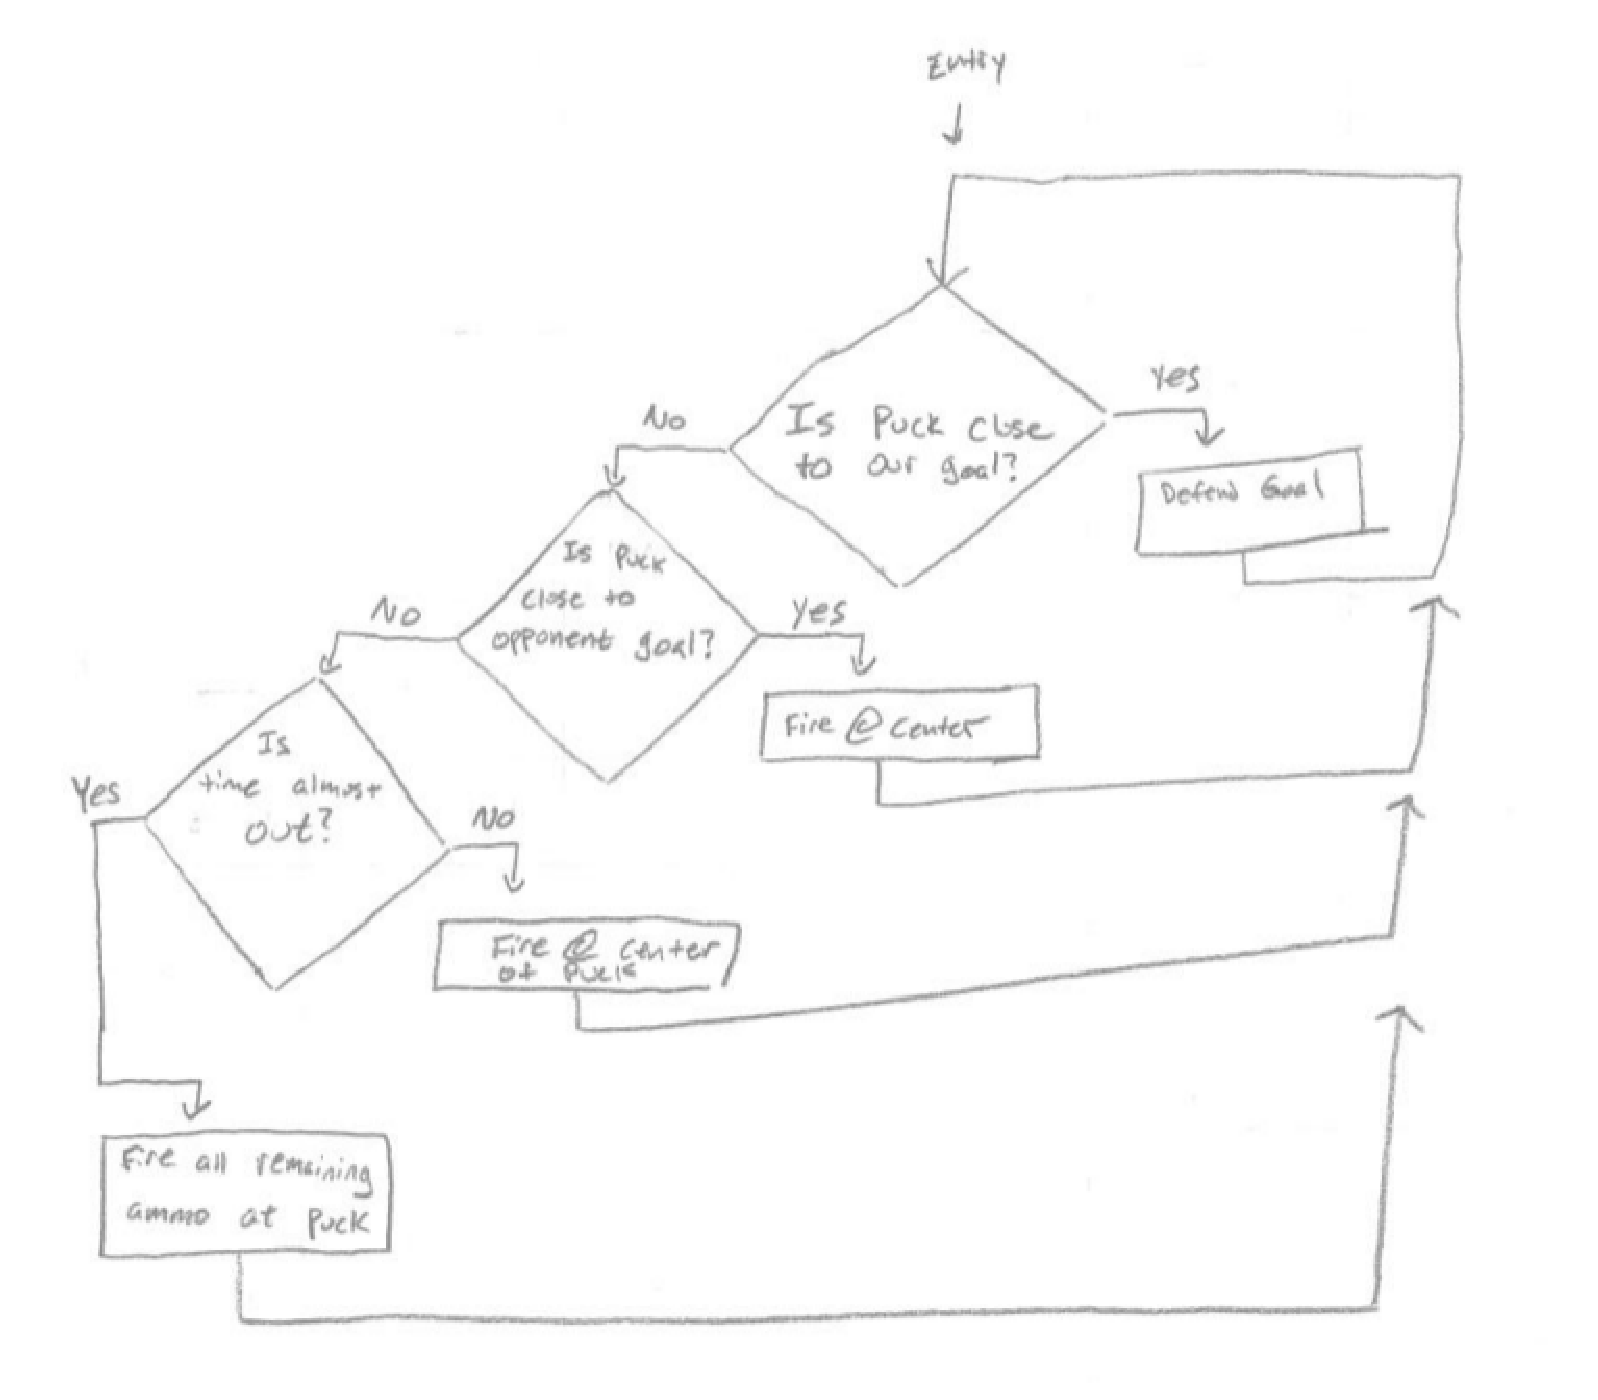
\includegraphics[width=0.8\textwidth]{./decision_tree.eps}
  \caption{Simple decision tree for implementing basic game engine.}
  \label{figure_decisions}
\end{figure}

\subsection{Projectile Aim \& Fire Mechanism}
The Projectile Aim and Fire Mechanism is responsible for translating target
locations delivered by the game engine into the physical action of firing a 
projectile.  The firing mechanism uses compressed air to propel the BBs from a
short cylindrical tube.  The compressed air is fired using an electronically
actuated valve, which is controlled by a microcontroller that is interfaced 
with a controlling PC or FPGA.  The firing direction is controlled by a stepper
motor that is also driven by the microcontroller.  The microcontroller uses a
loop-back sensor (encoder, potentiometer) to sense the current firing vector of
the cannon.  The game engine will provide the new firing vector to the
microcontroller, which will then position the stepper motor to the correct
location.  Figure \ref{figure_fire_block} shows the basic block diagram for
the Projectile Aim \& Fire Mechanism.


\begin{figure}[h!]
  \centering
  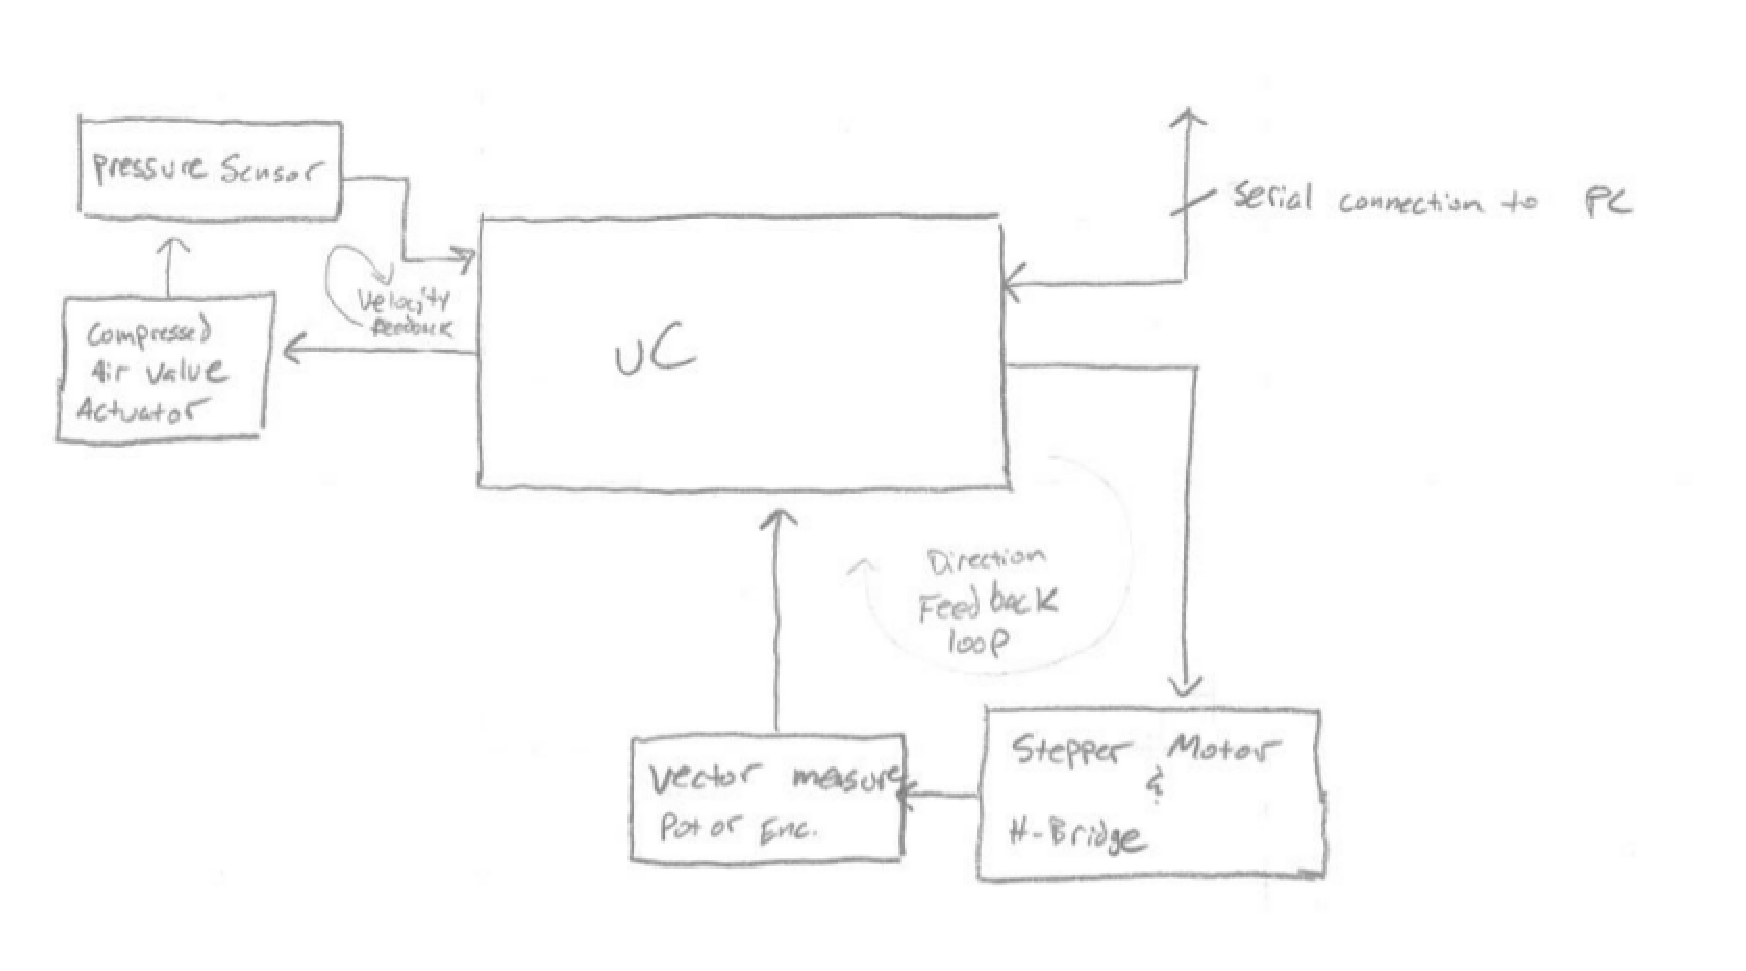
\includegraphics[width=0.8\textwidth]{./motor_block_diag.eps}
  \caption{Block diagram showing the Aim \& Fire Mechanism}
  \label{figure_fire_block}
\end{figure}



\section{Team Member Responsibilities}
As the teams have not yet been finalized, I can only speculate on my specific
role.  However, because of my programming skills, I will most likely be
responsible for the computer vision (Targeting/Tracking) portion of the project.
I will also offer assistance with the microcontroller integration, which will
require establishing communication channels between both the controlling PC and
the motor(s)/actuators.  The basic design/implementation of the game engine
will most likely be my responsibility as well, however the strategy component
of the design will most likely be a team-effort.

\section{Next Steps}
As soon as the teams are finalized (and possibly before), I will be meeting with
my team to discuss the various design ideas that we each had.  At this point,
we will divide the work among us, and get started.  I have already begun
some preliminary research into various computer vision techniques, as 
I anticipate that this will be the most challenging software component for 
me to implement; due mainly to my lack of experience in the area.


\end{document}
